% mrv-affectation.tex

%-------------------------------------------------------------------------
\section{Rappels de cours}\label{affectation:cours}
%-------------------------------------------------------------------------

%-------------------------------------------------------------------------
\subsection{Variables}\label{affectation:cours:variables}
%-------------------------------------------------------------------------

En informatique, l'essentiel du travail effectué par un programme d'ordinateur consiste 
à manipuler des données. Ces données peuvent être très diverses et
pour accéder à ces données, il est pratique de les nommer plutôt que de connaître
explicitement leur adresse en mémoire. 

Une donnée apparaît ainsi sous un nom de variable :
on dit que la variable dénote une valeur (fait référence à une valeur).
Pour la machine, il s'agit d'une référence 
désignant une adresse mémoire, c'est-à-dire un emplacement précis dans 
la mémoire vive où est stockée une valeur bien déterminée qui est la donnée 
proprement dite.
En informatique, une variable possède à un moment donné une valeur et une seule.

Une variable peut ainsi être vue comme une case en mémoire vive, que le programme 
va repérer par une étiquette (une adresse ou un nom). Pour avoir accès au contenu de la case
(la valeur de la variable), il suffit de la désigner par son étiquette : c'est-à-dire 
soit par son adresse en mémoire, soit par son nom.

\begin{definition}[variable]
Une variable est un objet informatique qui associe un nom à une valeur 
qui peut éventuellement varier au cours du temps.
\end{definition}

Les noms de variables sont des identificateurs arbitraires, de préférence assez courts mais aussi 
explicites que possible, de manière à exprimer clairement ce que la variable est censée 
référencer (la sémantique de la donnée référencée par la variable). 
Les noms des variables doivent en outre obéir à quelques règles simples :
\begin{itemize}
\item Un nom de variable est une séquence de lettres (a\ldots  z , A\ldots  Z) 
		et de chiffres (0\ldots  9), qui
      	doit toujours commencer par une lettre.\\
      	Exemples : \texttt{x}, \texttt{x1}, \texttt{x2}, \texttt{theta}, \texttt{tmp},
      	\texttt{mot}, \texttt{pression}, \texttt{longitude} 
\item Seules les lettres ordinaires sont autorisées. Les lettres accentuées, les cédilles, 
		les espaces, les caractères spéciaux tels que {\tt \$}, {\tt \#}, {\tt @}, etc. 
		sont interdits, à l'exception du caractère {\tt \_} (souligné).\\
		Exemples : \texttt{vitesse\_angulaire}, \texttt{une\_variable},
		\texttt{une\_autre\_variable}
\item La « casse » est significative : les caractères majuscules et minuscules sont 
		distingués. Ainsi,
      	{\tt python}, {\tt Python}, {\tt PYTHON} sont des variables différentes. 
\item Par convention, on écrira l'essentiel des noms de variable en caractères minuscules 
	(y compris la première lettre). 
	On n'utilisera les majuscules qu'à l'intérieur même du nom  
	pour en augmenter éventuellement la lisibilité, comme dans {\tt programmePython} ou
	{\tt angleRotation}.
	Une variable dont la valeur associée ne varie pas au cours du programme 
	(on parle alors de constante)
	pourra être écrite entièrement en majuscule, par exemple \texttt{PI} ($\pi = 3.14$) ou
	\texttt{ROUGE} (la couleur rouge).
\item Le langage lui-même peut se réserver quelques noms comme c'est le cas pour {\sc Python}
	(Table \ref{tab:python:mots-cles}).
	Ces mots réservés ne peuvent donc pas être utilisés comme noms de variable.

	\begin{table}[ht]
	$$\begin{tabular}{|lllll|}
	\hline
	\multicolumn{5}{|c|}{\rm{\textbf{Mots réservés en \python}}}\\
	\hline
	\tt False      & \tt class      & \tt finally    & \tt is         & \tt return\\
	\tt None       & \tt continue   & \tt for        & \tt lambda     & \tt try\\
	\tt True       & \tt def        & \tt from       & \tt nonlocal   & \tt while\\
	\tt and        & \tt del        & \tt global     & \tt not        & \tt with\\
	\tt as         & \tt elif       & \tt if         & \tt or         & \tt yield\\
	\tt assert     & \tt else       & \tt import     & \tt pass		  & \\
	\tt break      & \tt except     & \tt in         & \tt raise      & \\\hline
	\end{tabular}$$
	\caption{Mots réservés en \python{} 3}
	\label{tab:python:mots-cles}
	\end{table}

\end{itemize}

%-------------------------------------------------------------------------
\subsection{Attribuer une valeur}\label{affectation:cours:definition}
%-------------------------------------------------------------------------
Une fois nommée, il est souvent nécessaire de modifier la valeur de la donnée
référencée par une variable. C'est le rôle de l'instruction d'affectation.

\begin{definition}[affectation]
L'affectation est l'opération qui consiste à attribuer une valeur à une variable.
\end{definition}

L'instruction d'affectation est notée {\tt =} en {\sc Python} : \texttt{variable = valeur}. 
Le nom de la variable à modifier est placé dans le membre de gauche du signe {\tt =}, 
la valeur qu'on veut lui attribuer dans le membre de droite. 
Le membre de droite de l'affectation est d'abord évalué sans être modifié
puis la valeur obtenue est affectée à la variable dont le nom est donné dans 
le membre de gauche de l'affectation; ainsi, cette opération ne modifie 
que le membre de gauche de l'affectation.
L'affectation n'est donc pas une opération commutative (symétrique) : 
({\tt a = b}) $\neq$ ({\tt b = a}). 
En effet, avec l'instruction {\tt a = b},
on modifie la valeur de {\tt a} et pas celle de {\tt b} tandis qu'avec l'instruction
{\tt b = a}, on modifie {\tt b} mais pas {\tt a}.


Le membre de droite peut être une constante ou une expression évaluable.
\begin{description}
\item[\texttt{variable = constante}] : La constante peut être d'un type quelconque :
	entier, réel, booléen, chaîne de caractères, tableau, matrice, dictionnaire\ldots\ 
	comme le suggèrent les exemples suivants.

	\begin{minipage}[t]{5.5cm}
	\begin{verbatim}booleen = False
	entier = 3
	reel = 0.0
	chaine = "salut"
	tableau = [5,2,9,3]
	matrice = [[1,2],[6,7]]
	nUplet = 4,5,6
	dictionnaire = {}
	\end{verbatim}
	\end{minipage}
	\hfill
	\begin{minipage}[t]{9cm}
	\begin{verbatim}
	autreBooleen = True
	autreEntier = -329
	autreReel = -5.4687e-2
	autreChaine = 'bonjour, comment ça va ?'
	autreTableau = ['a',[6,3.14],[x,y,[z,t]]]
	autreMatrice = [[1,2],[3,4],[5,6],[7,8]]
	autreNUplet = "e",True,6.7,3,"z"
	autreDictionnaire = {"a":7, "r":-8}
	\end{verbatim}
	\end{minipage}
	\vspace*{2mm}
	
	En \python, la valeur que l'on affecte à une variable impose dynamiquement
	le type de la variable (Table \ref{tab:python:types-de-base}). Ainsi,
	si l'on affecte la valeur \texttt{3.14} à la variable \texttt{x} (\texttt{x = 3.14}), 
	celle-ci dénote alors un réel (type \texttt{float} en \python); si par contre,
	on lui affecte la valeur \texttt{'salut'} (\texttt{x = 'salut'}), 
	elle dénote alors une chaîne de caractères (type \texttt{str} en \python).

\begin{table}[ht]
$$\begin{tabular}{|lll|}
\hline
\multicolumn{3}{|c|}{\textbf{Types de base en \python}}\\
\hline
nom & type & exemples \\
\hline
booléen 		& \tt bool 	& {\tt False}, {\tt True}\\
entier  		& \tt int  	& \tt 3, -7\\
réel    		& \tt float & \tt 3.14, 7.43e-3\\
chaîne  		& \tt str 	& \tt 'salut', "l'eau"\\
n-uplet 		& \tt tuple & \tt 1,2,3\\
liste   		& \tt list  & \tt [1,2,3] \\
dictionnaire 	& \tt dict 	& \tt \{'a':4, 'r':8\}\\
\hline
\end{tabular}$$
\caption{Principaux types de base en \python}
\label{tab:python:types-de-base}
\end{table}

\item[\texttt{variable = expression}] : L'expression peut être n'importe quelle 
	expression évaluable telle qu'une opération logique ({\tt x = True or False and not True}), 
	une opération arithméti\-que ({\tt x = 3 + 2*9 - 6*7}), 
	un appel de fonction ({\tt y = sin(x)}) ou 
	toute autre combinaison évaluable
	({\tt x = (x != y) and (z + t >= y) or (sin(x) < 0)}).
	
	\begin{minipage}[t]{5.5cm}
	\begin{verbatim}
	reste = a%b
	somme = n*(n+1)/2
	delta = b*b - 4*a*c
	surface = pi*r**2
	\end{verbatim}
	\end{minipage}
	\hfill
	\begin{minipage}[t]{9cm}
	\begin{verbatim}
	quotient = a/b
	sommeGeometrique =  s = a*(b**(n+1)-1)/(b-1)
	racine = (-b + sqrt(delta))/(2*a)
	volume = surface * hauteur
	\end{verbatim}
	\end{minipage}
	\vspace*{2mm}

	L'expression du membre de droite peut faire intervenir la variable 
	du membre de gauche comme dans {\tt i = i+1}. Dans cet exemple, on évalue
	d'abord le membre de droite ({\tt i+1}) puis on attribue la valeur obtenue au
	membre de gauche ({\tt i}); ainsi, à la fin de cette affectation, la valeur de {\tt i}
	a été augmentée de {\tt 1} : on dit que {\tt i} a été incrémenté de {\tt 1}
	et on parle d'incrémentation de la variable {\tt i}. 
	Le langage \python\ propose un opérateur d'incrémentation ({\tt +=})
	et d'autres opérateurs d'affectation qui peuvent toujours se ramener
	à l'utilisation de l'opérateur {\tt =}, l'opérateur d'affectation de base
	(Table \ref{tab:python:affectations}).
\end{description}
	
	\begin{table}[ht]
	$$\begin{tabular}{|lll|}
	\hline
	\multicolumn{3}{|c|}{\textbf{Affectations en \python}}\\
	\hline
	\tt a = b  & & \\ 
	\hline	
	\tt a += b & $\equiv$  & \tt a = a + b \\
	\tt a -= b & $\equiv$  & \tt a = a - b \\	
	\tt a *= b & $\equiv$  & \tt a = a * b \\ 	
	\tt a /= b & $\equiv$  & \tt a = a / b \\ 	
	\tt a \%= b& $\equiv$ & \tt a = a \% b \\	
	\tt a **= b& $\equiv$  & \tt a = a ** b \\
	\hline
	\end{tabular}$$
	\caption{Affectations en \python}
	\label{tab:python:affectations}
	\end{table}

Avec l'exemple de l'incrémentation ({\tt i = i+1}), 
on constate que l'affectation est une opération 
typiquement informatique qui se distingue de l'égalité mathématique. En effet,
en mathématique une expression du type {\tt i = i+1} se réduit en
{\tt 0 = 1} ! Alors qu'en informatique, l'expression {\tt i = i+1} conduit à ajouter {\tt 1} 
à la valeur de {\tt i} (évaluation de l'expression {\tt i+1}), puis à donner cette
nouvelle valeur à {\tt i} (affectation).
L'affectation peut ainsi être vue comme un opérateur temporel : il y a un avant et
un après l'affectation.

L'affectation a donc pour effet de réaliser plusieurs opérations en mémoire :
\begin{itemize}
\item créer et mémoriser une valeur particulière,
\item créer et mémoriser un nom de variable,
\item établir un lien (par un système interne de pointeurs) entre le nom de la variable 
	et l'emplacement mémoire de la valeur correspondante,
\item attribuer un type déterminé à la variable.
\end{itemize}

%-------------------------------------------------------------------------
\subsection{Séquences d'affectations}\label{affectation:cours:sequences}
%-------------------------------------------------------------------------
Un apprenti informaticien a qui on demandait d'échanger ({\em swap}) les valeurs
de 2 variables {\tt x} et {\tt y} proposa la suite d'instructions suivante :
\vspace*{2mm}

\noindent\begin{minipage}{2cm}
\begin{Verbatim}
x = y
y = x
\end{Verbatim}
\end{minipage}
\hfill
\begin{minipage}{13cm}
et eut la désagréable surprise de constater que les valeurs des variables 
n'étaient pas permutées après cette séquence d'affectations.
\end{minipage}
\vspace*{2mm}

\noindent En effet, pour fixer les idées supposons qu'initialement {\tt x = 10} et {\tt y = 20}.
L'affectation {\tt x = y} conduit à évaluer {\tt y} puis à attribuer la valeur de {\tt y} ({\tt 20})
à {\tt x} : {\tt x} vaut maintenant {\tt 20}. La deuxième affectation ({\tt y = x}) 
commence par évaluer {\tt x} puis à attribuer la valeur de {\tt x} ({\tt 20}) à {\tt y}.
Après ces 2 affectations, {\tt x} et {\tt y} sont donc identiques et non permutées! 
Pour effectuer la permutation, l'apprenti informaticien aurait pu utiliser une variable 
temporaire (que nous nommerons {\tt tmp}) et exécuter la séquence d'instructions suivante :
\vspace*{2mm}

\noindent\begin{minipage}{2cm}
\begin{Verbatim}
tmp = x
x = y
y = tmp
\end{Verbatim}
\end{minipage}
\hfill
\begin{minipage}{13cm}
La première affectation ({\tt tmp = x}) permet de stocker la valeur initiale de {\tt x} ({\tt 10}),
la deuxième ({\tt x = y}) attribue à {\tt x} la valeur de {\tt y} ({\tt 20}) et la troisième ({\tt y = tmp})
attribue à {\tt y} la valeur de {\tt tmp}, c'est-à-dire la valeur initiale de {\tt x} ({\tt 10}).
Ainsi, les valeurs finales de {\tt x} et {\tt y} ({\tt 20} et {\tt 10}) sont bien permutées 
par rapport aux valeurs initiales ({\tt 10} et {\tt 20}).
\end{minipage}
\vspace*{2mm}

\noindent En \python, les n-uplets permettent d'écrire plus simplement la permutation
de deux variables : \texttt{x, y = y, x} .

L'exemple précédent de la permutation illustre la possibilité
de réaliser des calculs plus ou moins compliqués à l'aide d'une séquence 
d'affectations bien choisies. 
Mais ce sont les tests (Chapitre \ref{instructions:tests}) 
et les boucles  (Chapitre \ref{instructions:boucles}) 
qui nous permettront d'aborder des algorithmes réutilisables et plus robustes, 
en améliorant l'expressivité du programmeur.

Les sections suivantes de ce chapitre mettent en \oe uvre l'instruction d'affectation
dans différents domaines thématiques.

%-------------------------------------------------------------------------
\section{Vie courante : prix d'un livre}\label{affectation:vie-courante}
%-------------------------------------------------------------------------

\subsection{Objectifs}\label{affectation:vie-courante:objectif}
\begin{description}
\item[Principal : ] mettre en \oe uvre l'instruction d'affectation.
\item[Secondaire :] déterminer le prix d'un livre compte-tenu de réductions et des taxes.
\end{description}

\subsection{Syntaxe \python}\label{affectation:vie-courante:python}

\begin{description}
\item[\texttt{variable = expression}]\mbox{}
\end{description}

\subsection{Enoncé}\label{affectation:vie-courante:enonce}
Un libraire propose une réduction de 3.5\% sur le prix hors taxes (HT) 
d'un livre à 12.35 \euro{} HT.
Sachant que la taxe sur la valeur ajoutée (TVA) sur les livres est de 5.5\%, 
proposer une instruction de type « affectation » qui permettra de calculer 
le prix final toutes taxes comprises (TTC) pour le client.

\subsection{Méthode}\label{affectation:vie-courante:methode}
Pour expliciter la méthode qui nous permettra de résoudre un ensemble de problèmes 
équivalents et en particulier le problème posé dans l'énoncé, on commence par s'abstraire 
des données spécifiques, en particulier numériques, pour ne considérer que les variables associées. 
Ainsi, on ne s'intéressera pas à la valeur « 12.35 \euro~» mais à ce qu'elle qualifie : 
c'est-à-dire le prix hors taxes du livre, le « livre » étant lui-même un cas particulier de produit.
Et ainsi de suite pour chaque donnée spécifique du problème posé à laquelle on attribuera un nom.

Il s'agit donc ici de calculer le prix TTC (noté \texttt{ttc}) d'un produit
connaissant son prix HT (noté \texttt{ht}), la TVA (notée \texttt{tva} et
exprimée sous la forme d'un pourcentage) sur ce type de produit et 
la réduction éventuelle (notée \texttt{r} et exprimée sous la forme d'un 
pourcentage du prix HT) proposée par le vendeur sur ce produit.

Sachant qu'une réduction se soustrait du prix HT initial et 
qu'une taxe s'ajoute au prix hors taxes,
on a ainsi : \texttt{ttc = ht*(1-r/100)*(1+tva/100)} .

\subsection{Résultat}\label{affectation:vie-courante:resultat}
Appliquer la méthode précédente revient simplement ici à initialiser les variables
\texttt{ht}, \texttt{r} et \texttt{tva} aux données du problème particulier.

On applique donc la méthode précédente au livre à 12.35 \euro{} HT (\texttt{ht = 12.35}) 
avec une réduction de 3.5\% (\texttt{r = 3.5}) et une TVA à 5.5\% (\texttt{tva = 5.5}).

\noindent\begin{minipage}{7cm}
Compte-tenu de ces valeurs, le code \python{} ci-contre
permet de calculer le prix final TTC demandé (12.57 \euro).
\end{minipage}
\hfill
\begin{minipage}{8cm}
\begin{lstlisting}[caption=\textbf{prix d'un livre}]
ht, r, tva = 12.35, 3.5, 5.5
ttc = ht*(1-r/100)*(1+tva/100)
\end{lstlisting}
\tt\footnotesize
>>> ttc\\
12.57322625
\end{minipage}
\vspace*{2mm}

Remarque : on n'a pas cherché à effectuer « à la main » les calculs numériques :
\python{} les fera mieux que nous; et surtout, on n'a pas cherché non plus à 
particulariser la $2^{\grave eme}$ ligne du code en \texttt{ttc = 12.35*0.965*1.055} :
la forme plus abstraite \texttt{ttc = ht*(1-r/100)*(1+tva/100)} restera identique pour 
tout autre type de produit, de réduction et de TVA. 

\subsection{Vérification}\label{affectation:vie-courante:verification}
Une vérification possible est liée à l'ordre de grandeur du résultat obtenu.

Compte-tenu des taux respectifs de la réduction et de la TVA (\texttt{r} $<$ \texttt{tva}),
le prix final sera supérieur au prix HT et inférieur au prix TTC sans réduction.
On vérifie bien cette propriété : $12.35 < 12.57 < 12.35\cdot(1+0.055) = 13.03$, le
prix obtenu ici (12.57 \euro) a donc de fortes chances d'être correct.

Une autre vérification nécessaire concerne la généricité de la méthode : on doit 
pouvoir l'appliquer à d'autres exemples de produits, de taux de TVA ou encore de réductions.
C'est l'objet de la section \ref{affectation:vie-courante:genericite} suivante.

\subsection{Généricité}\label{affectation:vie-courante:genericite}
Pour tester la généricité de la méthode précédente, 
calculer à l'aide du code \python{} précédent, les prix TTC dans les cas suivants.
\begin{enumerate}
\item Un cinéma propose des places de cinéma, taxées à 7\%, avec une réduction de 44.75\% 
	sur le prix HT de 9.30\euro. Quel est le prix de la place de cinéma pour le client ?
\item Une grande surface vend 3 tablettes de chocolat de 100g chacune pour le prix de 2
	sachant que le chocolat, soumis à une TVA de 19.6\%, est à 9.90\euro/kg.
	Quel est le prix des 3 tablettes de chocolat pour le client ?
\end{enumerate}

\subsection{Entraînement}\label{affectation:vie-courante:entrainement}
Dans le même esprit, utiliser une instruction d'affectation pour déterminer :
\begin{enumerate}
\item la durée totale du trajet \textsc{Brest}-\textsc{Rennes}, 
	en car de \textsc{Brest} (10h00) à \textsc{Quimper} (11h20)
	puis en \textsc{Tgv} de \textsc{Quimper} (11h40) à \textsc{Rennes} (13h55),
\item l'augmentation de la facture de fuel d'un particulier pour une cuve de 1400 l 
	si le fuel domestique, anciennement à 0.938 \euro/l, augmente de 5\%.
\end{enumerate}

%-------------------------------------------------------------------------
\section{Jeux : lancer de dés}
%-------------------------------------------------------------------------

\subsection{Objectif}\label{affectation:jeux:objectif}
\begin{description}
\item[Principal : ] mettre en \oe uvre l'instruction d'affectation.
\item[Secondaire :] simuler un lancer de dés.
\end{description}

\subsection{Syntaxe \python}\label{affectation:jeux:python}
\begin{description}
\item[\texttt{variable = expression}]\mbox{}

\item[\texttt{range(start,stop,step)}] retourne une liste d'entiers compris 
	entre \texttt{start} inclus (= 0 par défaut) et \texttt{stop} exclu,
	par pas de \texttt{step} (= 1 par défaut).
\vspace*{2mm}

\begin{minipage}[t]{7cm}\footnotesize
\begin{Verbatim}
>>> range(0,4,1)
[0, 1, 2, 3]
>>> range(0,4)
[0, 1, 2, 3]
>>> range(4)
[0, 1, 2, 3]
\end{Verbatim}
\end{minipage}
\hfill
\begin{minipage}[t]{7cm}\footnotesize
\begin{Verbatim}
>>> range(3)
[0, 1, 2]
>>> range(3,9,2)
[3, 5, 7]
>>> range(7,0,-1)
[7, 6, 5, 4, 3, 2, 1]
\end{Verbatim}
\end{minipage}
\vspace*{2mm}

\item[\texttt{randrange(start,stop,step)}] retourne un élément choisi aléatoirement
	dans la liste retournée par la fonction \texttt{range(start,stop,step)}.
	Il est nécessaire d'importer la fonction \texttt{randrange} depuis le module \texttt{random} :
	\texttt{from random import randrange}.
\vspace*{2mm}
	
\begin{minipage}{7cm}\footnotesize
\begin{Verbatim}
>>> from random import randrange
>>> randrange(0,4,1)
1
>>> randrange(0,4)
0
>>> randrange(4)
2
\end{Verbatim}
\end{minipage}
\hfill
\begin{minipage}{7cm}\footnotesize
\begin{Verbatim}
>>> from random import randrange
>>> randrange(3)
2
>>> randrange(3,9,2)
5
>>> randrange(7,0,-1)
3
\end{Verbatim}
\end{minipage}
\end{description}

\subsection{Enoncé}\label{affectation:jeux:enonce}
Proposer une instruction de type « affectation » qui permettra
de simuler un lancer de dé à 6 faces. 
On pourra utiliser la fonction \texttt{randrange} 
de la section \ref{affectation:jeux:python} précédente.

\subsection{Méthode}\label{affectation:jeux:methode}
Pour expliciter la méthode qui nous permettra de résoudre un ensemble de problèmes 
équivalents et en particulier le problème posé dans l'énoncé, on commence par s'abstraire 
des données spécifiques, en particulier numériques, pour ne considérer que les variables associées. 
Ainsi, on généralisera le « dé à six faces » en un tirage aléatoire d'un entier compris entre deux 
autres entiers à chacun desquels on attribuera un nom.

Il s'agit donc ici de déterminer un entier \texttt{de} compris entre 2 nombres \texttt{min} et \texttt{max}
inclus, par pas de \texttt{step}.
On peut donc directement utiliser la fonction \texttt{randrange} :\\
\texttt{de = randrange(min,max+1,step)}.

\subsection{Résultat}\label{affectation:jeux:resultat}
Appliquer la méthode précédente revient simplement ici à initialiser les variables
\texttt{min}, \texttt{max} et \texttt{step} aux données du problème particulier.

On applique donc la méthode précédente au dé à 6 faces : \texttt{min = 1}, \texttt{max = 6} et 
\texttt{step = 1}.

\noindent\begin{minipage}{7cm}
Compte-tenu de ces valeurs, le code \python{} ci-contre
permet de simuler un lancer de dé à 6 faces.
\end{minipage}
\hfill
\begin{minipage}{8cm}
\begin{lstlisting}[caption=\textbf{lancer de dé}]
from random import randrange
min, max, step = 1, 6, 1
de = randrange(min,max+1,step)
\end{lstlisting}
\tt\footnotesize
>>> de\\
4
\end{minipage}
\vspace*{2mm}

Remarque : on n'a pas cherché à 
particulariser et simplifier la $3^{\grave eme}$ ligne du code en \texttt{de = randrange(1,7)} :
la forme plus abstraite \texttt{de = randrange(min,max+1,step)} restera identique pour 
tout autre type de « dé ». 

\subsection{Vérification}\label{affectation:jeux:verification}
La fonction \texttt{randrange} est une fonction d'un module standard de \python{} 
(le module \texttt{random}) : 
il y a peu de doutes sur le fait qu'elle fonctionne correctement.
On vérifiera simplement ici que le code proposé ne « sort » pas des valeurs
inférieures à 1 ou supérieures à 6 en le testant plusieurs fois de suite ou, 
au contraire, « sort » bien de temps en temps les valeurs extrêmes 1 et 6.
\vspace*{2mm}
	
\begin{minipage}[t]{7cm}\footnotesize
\begin{Verbatim}
>>> from random import randrange
>>> min, max, step = 1, 6, 1
>>> de = randrange(min,max+1,step)
>>> de
2
>>> de = randrange(min,max+1,step)
>>> de
6
>>> de = randrange(min,max+1,step)
>>> de
3
>>> de = randrange(min,max+1,step)
>>> de
3
\end{Verbatim}
\end{minipage}
\hfill
\begin{minipage}[t]{7cm}\footnotesize
\begin{Verbatim}
>>> from random import randrange
>>> min, max, step = 1, 6, 1
>>> de = randrange(min,max+1,step)
>>> de
1
>>> de = randrange(min,max+1,step)
>>> de
3
>>> de = randrange(min,max+1,step)
>>> de
5
>>> de = randrange(min,max+1,step)
>>> de
2
\end{Verbatim}
\end{minipage}
\vspace*{2mm}

Une autre vérification nécessaire concerne la généricité de la méthode : on doit 
pouvoir l'appliquer à d'autres exemples de « dés ».
C'est l'objet de la section \ref{affectation:jeux:genericite} suivante.

\subsection{Généricité}\label{affectation:jeux:genericite}
Pour tester la généricité de la méthode précédente, 
simuler, à l'aide du code \python{} précédent, le tirage aléatoire :
\begin{enumerate}
\item d'une carte d'un jeu de 32 cartes,
\item d'une boule du \textsc{Loto}.
\end{enumerate}

\subsection{Entraînement}\label{affectation:jeux:entrainement}
Dans le même esprit, utiliser l'affectation pour :
\begin{enumerate}
\item simuler le tirage aléatoire d'une carte d'une couleur donnée 
	($\spadesuit$, $\heartsuit$, $\diamondsuit$ ou $\clubsuit$) issue 
	d'un jeu de 32 cartes, la couleur étant elle-même tirée au sort;
\item calculer la somme de deux dés tirés chacun aléatoirement.
\end{enumerate}

%-------------------------------------------------------------------------
\section{Textes : longueurs de chaînes de caractères}
%-------------------------------------------------------------------------

\subsection{Objectif}\label{affectation:textes:objectif}
\begin{description}
\item[Principal : ] mettre en \oe uvre l'instruction d'affectation.
\item[Secondaire :] comparer les longueurs de deux chaînes de caractères.
\end{description}

\subsection{Syntaxe \python}\label{affectation:textes:python}
\begin{description}
\item[\texttt{variable = expression}]\mbox{}
\item[\texttt{len(s)}] retourne le nombre d'éléments (la longueur, \emph{length}) de la séquence \texttt{s}.
\item[\texttt{x in s}] teste si \texttt{x} est un élément de (appartient à, est dans) la séquence \texttt{s}.
\item[\texttt{s[i]}] retourne l'élément de rang \texttt{i} dans la séquence \texttt{s}.

	Attention ! Par convention, les indices des éléments dans une séquence commencent à {\tt 0}.
	Le premier élément a pour indice {\tt 0} ({\tt s[0]}), le deuxième l'indice {\tt 1}
	({\tt s[1]}), le troisième l'indice {\tt 2} ({\tt s[2]}) et ainsi de suite jusqu'au 
	dernier qui a l'indice {\tt n-1} ({\tt s[n-1]}) si {\tt n} est le nombre d'éléments 
	dans la séquence ({\tt n == len(s)}).
\item[\texttt{s[i:j]}] retourne la séquence comprise entre les rangs \texttt{i} inclus et 
	\texttt{j} exclu de la séquence \texttt{s}.
\item[\texttt{s1 + s2}] retourne la séquence résultat de la concaténation (la mise bout à bout) des 
	deux séquences \texttt{s1} et \texttt{s2}.

\begin{minipage}[t]{4cm}
n-uplets :\footnotesize
\begin{Verbatim}
>>> s = 1,7,2,4
>>> type(s)
<type 'tuple'>
>>> len(s)
4
>>> 3 in s
False
>>> s[1]
7
>>> s[1:3]
(7, 2)
>>> s + (5,3)
(1, 7, 2, 4, 5, 3)
\end{Verbatim}
\end{minipage}
\hfill
\begin{minipage}[t]{4cm}
chaînes de caractères :\footnotesize
\begin{Verbatim}
>>> s = '1724'
>>> type(s)
<type 'str'>
>>> len(s)
4
>>> '3' in s
False
>>> s[1]
'7'
>>> s[1:3]
'72'
>>> s + '53'
'172453'
\end{Verbatim}
\end{minipage}
\hfill
\begin{minipage}[t]{4cm}
listes :\footnotesize
\begin{Verbatim}
>>> s = [1,7,2,4]
>>> type(s)
<type 'list'>
>>> len(s)
4
>>> 3 in s
False
>>> s[1]
7
>>> s[1:3]
[7, 2]
>>> s + [5,3]
[1, 7, 2, 4, 5, 3]
\end{Verbatim}
\end{minipage}

\end{description}

\subsection{Enoncé}\label{affectation:textes:enonce}
Proposer une instruction de type « affectation » qui permettra de tester si les deux chaînes de 
caractères \texttt{'bonjour'} et \texttt{'salut'} ont le même nombre d'éléments.
On pourra utiliser la fonction \texttt{len} de la section \ref{affectation:textes:python} précédente.

\subsection{Méthode}\label{affectation:textes:methode}
Pour expliciter la méthode qui nous permettra de résoudre un ensemble de problèmes 
équivalents et en particulier le problème posé dans l'énoncé, on commence par s'abstraire 
des données spécifiques, en particulier alphanumériques, pour ne considérer que les variables associées. 
Ainsi, on ne s'intéressera pas aux valeurs \texttt{'bonjour'} et \texttt{'salut'} mais
plutôt à ce qu'elles qualifient : deux chaînes de caractères auxquelles on attribuera un nom chacune.

Il s'agit donc ici de comparer les longueurs de deux chaînes \texttt{s1} et \texttt{s2}.
La longueur d'une chaîne de caractères s'obtient à l'aide de la fonction \texttt{len} : 
\texttt{len(s1)} ou \texttt{len(s2)}. On affecte donc simplement la comparaison 
\texttt{(len(s1) == len(s2))} à la réponse souhaitée :\\
\texttt{compar = (len(s1) == len(s2))};
\texttt{compar} prendra donc la valeur booléenne \texttt{True} ou \texttt{False}
selon que les longueurs sont égales ou non.

\subsection{Résultat}\label{affectation:textes:resultat}
Appliquer la méthode précédente revient simplement ici à initialiser les variables
\texttt{s1} et \texttt{s2} aux données du problème particulier.

On applique donc la méthode précédente avec les chaînes : \texttt{s1 = 'bonjour'}
et \texttt{s2 = 'salut'}.

\noindent\begin{minipage}{7cm}
Compte-tenu de ces valeurs, le code \python{} ci-contre
permet de comparer les longueurs de ces deux chaînes.
\end{minipage}
\hfill
\begin{minipage}{8cm}
\begin{lstlisting}[caption=\textbf{comparaison de longueurs}]
s1, s2 = 'bonjour', 'salut'
compar = (len(s1) == len(s2))
\end{lstlisting}
\tt\footnotesize
>>> compar\\
False
\end{minipage}
\vspace*{2mm}

Remarque : on n'a pas cherché à 
particulariser la $2^{\grave eme}$ ligne du code en \texttt{compar = (len('bon jour') == len('salut')} :
la forme plus abstraite \texttt{compar = (len(s1) == len(s2))} restera identique pour 
tout autre couple de chaînes. 

\subsection{Vérification}\label{affectation:textes:verification}
La vérification est ici immédiate puisqu'on peut calculer « à la main »
la longueur de chacune de ces chaînes : il y a 7 caractères dans la chaîne \texttt{'bonjour'}
et 5 dans la chaîne \texttt{'salut'}. Elles ne sont donc pas de la même longueur et le résultat
de la comparaison vaut \texttt{False} : ce que donne bien l'exécution du code précédent.

Une autre vérification nécessaire concerne la généricité de la méthode : 
on doit pouvoir l'appliquer à d'autres exemples de chaînes de caractères.
C'est l'objet de la section \ref{affectation:textes:genericite} suivante.

\subsection{Généricité}\label{affectation:textes:genericite}
Pour tester la généricité de la méthode précédente, déterminer, à l'aide du code \python{} précédent, 
si les chaînes suivantes sont de même longueur ou non :
\begin{enumerate}
\item la chaîne \texttt{'salut monde'} et la chaîne \texttt{'hello'} concaténée 
	avec la chaîne \texttt{'world'},
\item la chaîne \texttt{'démocratie'} et la chaîne \texttt{'anticonstitutionnellement'} considérée uniquement 
	entre les indices 4 et 8 inclus.
\end{enumerate}

\subsection{Entraînement}\label{affectation:textes:entrainement}
Dans le même esprit, utiliser l'affectation pour :
\begin{enumerate}
\item tester si la chaîne \texttt{'bonjour'} a moins de caractères que la chaîne \texttt{'au revoir'};
\item tester si la chaîne \texttt{'bonjour'} est plus petite que la chaîne \texttt{'au revoir'} 
	selon l'ordre lexicographique.
\end{enumerate}

%-------------------------------------------------------------------------
\section{Nombres : quotient et reste}
%-------------------------------------------------------------------------

\subsection{Objectif}\label{affectation:nombres:objectif}
\begin{description}
\item[Principal : ] mettre en \oe uvre l'instruction d'affectation.
\item[Secondaire :] calculer le quotient et le reste de la division entière de deux entiers.
\end{description}

\subsection{Syntaxe \python}\label{affectation:nombres:python}
\begin{description}
\item[\texttt{variable = expression}]\mbox{}
\item[\texttt{a//b}] retourne le quotient \texttt{q} de la division entière de 
	\texttt{a} par \texttt{b} : \texttt{a == b*q + r}.
\item[\texttt{a\%b}] retourne le reste \texttt{r} de la division entière de 
	\texttt{a} par \texttt{b} : \texttt{a == b*q + r}.
\end{description}

\subsection{Enoncé}\label{affectation:nombres:enonce}
Proposer une instruction de type « affectation » qui permettra de calculer le
quotient et le reste de la division entière $135\div 2$.
On pourra utiliser les opérateurs \texttt{//} et \texttt{\%} 
de la section \ref{affectation:nombres:python} précédente.

\subsection{Méthode}\label{affectation:nombres:methode}
Pour expliciter la méthode qui nous permettra de résoudre un ensemble de problèmes 
équivalents et en particulier le problème posé dans l'énoncé, on commence par s'abstraire 
des données spécifiques, en particulier numériques, pour ne considérer que les variables associées. 
Ainsi, on ne s'intéressera pas aux valeurs \texttt{135} et \texttt{2} mais
plutôt à ce qu'elles qualifient : deux entiers auxquels on attribuera un nom chacun.

Il s'agit donc ici de déterminer le quotient $q$ et le reste $r$ de la division
entière de deux nombres $a$ et $b$ : $a\div b$. On peut utiliser simplement les opérateurs
prédéfinis \texttt{//} et \texttt{\%} :\\
\texttt{q, r = a//b, a\%b}.

\subsection{Résultat}\label{affectation:nombres:resultat}
Appliquer la méthode précédente revient simplement ici à initialiser les variables
\texttt{a} et \texttt{b} aux données du problème particulier.

On applique donc la méthode précédente avec les entiers \texttt{a = 135}
et \texttt{b = 2}.

\noindent\begin{minipage}{7cm}
Compte-tenu de ces valeurs, le code \python{} ci-contre
permet de déterminer le quotient \texttt{q} et le reste 
\texttt{r} recherchés.
\end{minipage}
\hfill
\begin{minipage}{8cm}
\begin{lstlisting}[caption=\textbf{quotient et reste}]
a, b = 135, 2
q, r = a//b, a%b
\end{lstlisting}
\tt\footnotesize
>>> q, r\\
(67, 1)
\end{minipage}
\vspace*{2mm}

Remarque : on n'a pas cherché à 
particulariser la $2^{\grave eme}$ ligne du code en \texttt{q,r = 135//2, 135\%2};
la forme plus abstraite \texttt{q, r = a//b, a\%b}
restera identique pour tout autre division entière. 

\subsection{Vérification}\label{affectation:nombres:verification}
La vérification est ici immédiate puisqu'on peut calculer « de tête »
le quotient (67) et le reste (1) de la division entière de 135 par 2.

\noindent\begin{minipage}{7cm}
Une vérification plus générale consiste à vérifier la relation
\texttt{a == b*q + r} après avoir calculé \texttt{q} et \texttt{r}.
\end{minipage}
\hfill
\begin{minipage}{8cm}
\begin{lstlisting}
a, b = 135, 2
q, r = a//b, a%b
\end{lstlisting}
\tt\footnotesize
>>> a == b*q + r\\
True
\end{minipage}
\vspace*{2mm}

Une autre vérification nécessaire concerne la généricité de la méthode : 
on doit pouvoir l'appliquer à d'autres exemples de divisions entières.
C'est l'objet de la section \ref{affectation:nombres:genericite} suivante.

\subsection{Généricité}\label{affectation:nombres:genericite}
Pour tester la généricité de la méthode précédente, déterminer, à l'aide du code \python{} précédent, 
les quotients et restes des divisions suivantes :
\begin{enumerate}
\item $3553 \div 11$
\item $375375 \div 11$
\end{enumerate}

\subsection{Entraînement}\label{affectation:nombres:entrainement}
Dans le même esprit, utiliser l'affectation pour déterminer :
\begin{enumerate}
\item le nombre dont le quotient et le reste sont respectivement 13 et 7 
	lors d'une division par 17;
\item le diviseur de 345 si le quotient vaut 12 et le reste 9.
\end{enumerate}

%-------------------------------------------------------------------------
\section{Figures : distance entre deux points}\label{affectation:figures}
%-------------------------------------------------------------------------

\subsection{Objectif}\label{affectation:figures:objectif}
\begin{description}
\item[Principal : ] mettre en \oe uvre l'instruction d'affectation.
\item[Secondaire :] calculer la distance entre deux points du plan.
\end{description}

\subsection{Syntaxe \python}\label{affectation:figures:python}
\begin{description}
\item[\texttt{variable = expression}]\mbox{}
\item[\texttt{sqrt(x)}] (\emph{square root}) retourne la racine carrée de \texttt{x} ($\sqrt{x}$). 
	Il est nécessaire d'importer la fonction \texttt{sqrt} depuis le module \texttt{math} :
	\texttt{from math import sqrt}.
\end{description}

\subsection{Enoncé}\label{affectation:figures:enonce}
Proposer une instruction de type « affectation » qui permettra de calculer 
la distance entre les deux points $A$ et $B$ du plan ci-dessous.
$$
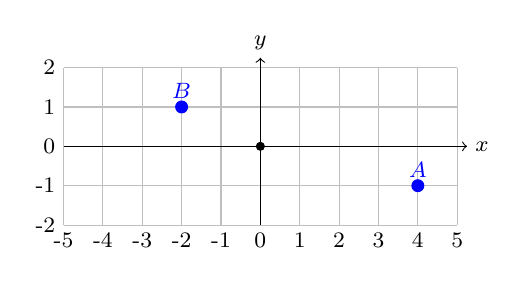
\begin{tikzpicture}[scale=0.5]\footnotesize
\draw[color=lightgray](-5,-2) grid[xstep=1,ystep=1] (5,2);
\foreach \x in {-5,-4,...,5} \draw(\x,-2) node[below]{\x};
\foreach \y in {-2,-1,...,2} \draw(-5,\y) node[left]{\y};
\filldraw(0,0) circle (0.1);
\draw[->] (-5,0) -- (5.25,0);
\draw (5.25,0) node[right]{$x$} ;
\draw[->] (0,-2) -- (0,2.25);
\draw (0,2.25) node[above]{$y$};
\filldraw[color=blue] (4,-1) circle (0.15);
\draw (4,-1) node[above,color=blue]{${A}$};
\filldraw[color=blue] (-2,1) circle (0.15);
\draw (-2,1) node[above,color=blue]{${B}$};
\end{tikzpicture}
$$

\subsection{Méthode}\label{affectation:figures:methode}
Pour expliciter la méthode qui nous permettra de résoudre un ensemble de problèmes 
équivalents et en particulier le problème posé dans l'énoncé, on commence par s'abstraire 
des données spécifiques, en particulier numériques, pour ne considérer que les variables associées. 
Ainsi, on ne s'intéressera pas aux valeurs des coordonnées (4,-1) ou (-2,1) mais
plutôt à ce qu'elles qualifient : deux points du plan auxquels on attribuera un nom chacun.

Il s'agit donc ici de déterminer la distance $d$ entre deux points $P_1$ et $P_2$ de $\mathbb{R}^2$
respectivement de coordonnées $(x_1,y_1)$ et $(x_2,y_2)$, à savoir $\displaystyle d = \sqrt{(x_2-x_1)^2 + (y_2-y_1)^2}$, d'où l'affectation :\linebreak
\texttt{d = sqrt((x2-x1)**2 + (y2-y1)**2)}.


\subsection{Résultat}\label{affectation:figures:resultat}
Appliquer la méthode précédente revient simplement ici à initialiser les variables
\texttt{x1}, \texttt{y1}, \texttt{x2} et \texttt{y2} aux données du problème particulier.

On applique donc la méthode précédente avec les coordonnées des points $A$ et $B$ :
\texttt{(x1, y1) = (4, -1)} et \texttt{(x2, y2) = (-2, 1)}.

\noindent\begin{minipage}{7cm}
Compte-tenu de ces valeurs, le code \python{} ci-contre
permet de calculer la distance \texttt{d} entre les points
$A$ et $B$ ($AB \approx 6.32$).
\end{minipage}
\hfill
\begin{minipage}{8cm}
\begin{lstlisting}[caption=\textbf{distance entre 2 points}]
from math import sqrt
x1, y1 = 4, -1
x2, y2 = -2, 1
d = sqrt((x2-x1)**2 + (y2-y1)**2)
\end{lstlisting}
\tt\footnotesize
>>> d\\
6.324555320336759
\end{minipage}
\vspace*{2mm}

Remarque : on n'a pas cherché à 
particulariser la $4^{\grave eme}$ ligne du code en « préparant » les calculs
« à la main » : \texttt{d = sqrt(40)};
la forme plus abstraite \texttt{d = sqrt((x2-x1)**2 + (y2-y1)**2)}
restera identique pour tout autre calcul de distance entre 2 points du plan. 

\subsection{Vérification}\label{affectation:figures:verification}
La vérification est ici immédiate puisqu'on peut vérifier rapidement que 
$d = \sqrt{40} \approx 6.32$.


\noindent\begin{minipage}{7cm}
Une autre vérification possible consiste à utiliser le module \texttt{turtle} (la tortue \logo)
de \python{} et sa fonction \texttt{distance} pour déterminer cette distance et 
la comparer au calcul précédent.\\
La différence \texttt{delta} étant nulle, on obtient bien les mêmes résultats.
\end{minipage}
\hfill
\begin{minipage}{8cm}
\begin{lstlisting}
from turtle import *
up()
goto(x1,y1)
down()
delta = d - distance(x2,y2)
\end{lstlisting}
\tt\footnotesize
>>> delta\\
0.0
\end{minipage}
\vspace*{2mm}

Une autre vérification nécessaire concerne la généricité de la méthode : 
on doit pouvoir l'appliquer à d'autres exemples de calculs de distances.
C'est l'objet de la section \ref{affectation:figures:genericite} suivante.

\subsection{Généricité}\label{affectation:figures:genericite}
Pour tester la généricité de la méthode précédente, déterminer, à l'aide du code \python{} précédent, 
les distances entre les points du diagramme ci-dessous : $AB$, $AC$, $AD$, $BC$, $BD$ et $CD$.
$$
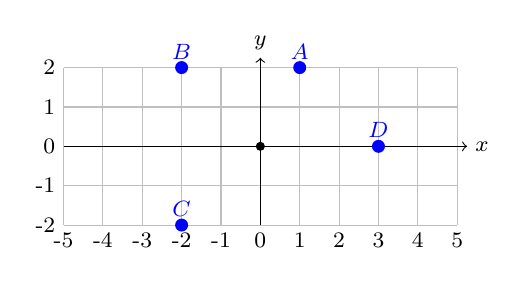
\begin{tikzpicture}[scale=0.5]\footnotesize
\draw[color=lightgray](-5,-2) grid[xstep=1,ystep=1] (5,2);
\foreach \x in {-5,-4,...,5} \draw(\x,-2) node[below]{\x};
\foreach \y in {-2,-1,...,2} \draw(-5,\y) node[left]{\y};
\filldraw(0,0) circle (0.1);
\draw[->] (-5,0) -- (5.25,0);
\draw (5.25,0) node[right]{$x$} ;
\draw[->] (0,-2) -- (0,2.25);
\draw (0,2.25) node[above]{$y$};
\filldraw[color=blue] (1,2) circle (0.15);
\draw (1,2) node[above,color=blue]{${A}$};
\filldraw[color=blue] (-2,2) circle (0.15);
\draw (-2,2) node[above,color=blue]{${B}$};
\filldraw[color=blue] (-2,-2) circle (0.15);
\draw (-2,-2) node[above,color=blue]{${C}$};
\filldraw[color=blue] (3,0) circle (0.15);
\draw (3,0) node[above,color=blue]{${D}$};
\end{tikzpicture}
$$

\subsection{Entraînement}\label{affectation:figures:entrainement}
Dans le même esprit, utiliser l'affectation pour :
\begin{enumerate}
\item vérifier que le triangle $ABC$ formé par les points $A$, $B$ et $C$ de la figure ci-dessus 
	(voir section \ref{affectation:figures:genericite} précédente) est un triangle rectangle;
\item déterminer les coordonnées d'un point $B$ sachant qu'il est situé à 4 unités de distance
	du point $A$ de coordonnées $(1,-2)$ et que l'angle entre l'axe des $x$ et $\vec{AB}$ 
	est de 60°.
\end{enumerate}

%-------------------------------------------------------------------------
\section{Mathématiques : produit scalaire}\label{affectation:maths}
%-------------------------------------------------------------------------

\subsection{Objectif}\label{affectation:maths:objectif}
\begin{description}
\item[Principal : ] mettre en \oe uvre l'instruction d'affectation.
\item[Secondaire :] calculer le produit scalaire de deux vecteurs.
\end{description}

\subsection{Syntaxe \python}\label{affectation:maths:python}
\begin{description}
\item[\texttt{variable = expression}]\mbox{}
\end{description}

\subsection{Enoncé}\label{affectation:maths:enonce}
On considère les 2 vecteurs $\vec{A}$ et $\vec{B}$ définis dans $\mathbb{R}^2$ 
comme le montre la figure ci-dessous.
$$
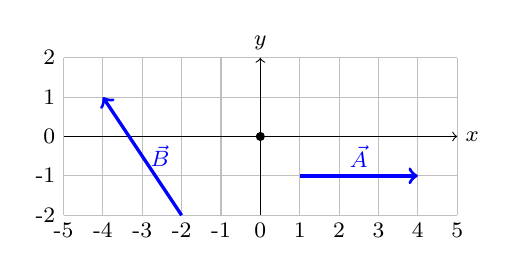
\begin{tikzpicture}[scale=0.5]\footnotesize
\draw[color=lightgray](-5,-2) grid[xstep=1,ystep=1] (5,2);
\foreach \x in {-5,-4,...,5} \draw(\x,-2) node[below]{\x};
\foreach \y in {-2,-1,...,2} \draw(-5,\y) node[left]{\y};
\filldraw(0,0) circle (0.1);
\draw[->] (-5,0) -- (5,0);
\draw (5,0) node[right]{$x$} ;
\draw[->] (0,-2) -- (0,2);
\draw (0,2) node[above]{$y$};
\draw[->,very thick,color=blue] (1,-1) -- (4,-1);
\draw[->,very thick,color=blue] (-2,-2) -- (-4,1);
\draw (2.5,-1) node[above,color=blue]{$\vec{A}$};
\draw (-3,-0.5) node[right,color=blue]{$\vec{B}$};
\end{tikzpicture}
$$
Proposer une instruction de type « affectation » qui permettra de calculer le produit scalaire
$\vec{A}\cdot\vec{B}$ de ces deux vecteurs.


\subsection{Méthode}\label{affectation:maths:methode}
Pour expliciter la méthode qui nous permettra de résoudre un ensemble de problèmes 
équivalents et en particulier le problème posé dans l'énoncé, on commence par s'abstraire 
des données spécifiques, en particulier numériques, pour ne considérer que les variables associées. 
Ainsi, on ne s'intéressera pas aux composantes numériques $(3,0)$ et $(-2,3)$ mais
plutôt à ce qu'elles qualifient : deux vecteurs du plan auxquels on attribuera un nom chacun.

Il s'agit donc ici de déterminer le produit scalaire $\vec{V}_1\cdot\vec{V}_2$ 
de 2 vecteurs $\vec{V}_1$ et $\vec{V}_2$ de $\mathbb{R}^2$
ayant pour composantes respectives $(x_1,y_1)$ et $(x_2,y_2)$. 
Par définition, ce produit scalaire est un réel $p$ qui a pour expression 
$p = x_1\cdot x_2 + y_1\cdot y_2$.

Connaissant les composantes respectivement $(x_1,y_1)$ et $(x_2,y_2)$ des 
vecteurs $\vec{V}_1$ et $\vec{V}_2$, 
on détermine le produit scalaire $p$ par une affectation simple : 
\texttt{p = x1*x2 + y1*y2} .

\subsection{Résultat}\label{affectation:maths:resultat}
On applique la méthode précédente aux vecteurs $\vec{V}_1 = \vec{A}$
et $\vec{V}_2 = \vec{B}$. Leurs composantes respectives se lisent directement 
sur la figure : 
$x_1 = (4) - (1) = 3$, $y_1 = (-1) - (-1) = 0$, 
$x_2 = (-4) - (-2) = -2$ et $y_2 = (1) - (-2) = 3$.

\noindent\begin{minipage}{7cm}
Compte-tenu de ces valeurs, le code ci-contre
permet de calculer le produit scalaire $\vec{A}\cdot\vec{B}$
demandé.
\end{minipage}
\hfill
\begin{minipage}{8cm}
\begin{lstlisting}[caption=\textbf{produit scalaire}]
x1, y1 = (4)-(1), (-1)-(-1)
x2, y2 = (-4)-(-2), (1)-(-2)
p = x1*x2 + y1*y2
\end{lstlisting}
\end{minipage}

Remarque : on n'a pas cherché à effectuer « à la main » les calculs numériques :
\python{} les fera mieux que nous; et surtout, on n'a pas cherché non plus à 
particulariser la $3^{\grave eme}$ ligne du code en \texttt{p = 3*(-2) + 0*3} :
la forme plus abstraite \texttt{p = x1*x2 + y1*y2} restera identique pour 
deux autres vecteurs quelconques de $\mathbb{R}^2$. 

\subsection{Vérification}\label{affectation:maths:verification}
Une autre manière de déterminer le produit scalaire est donnée par la formule
« géométrique~»~: $\vec{A}\cdot\vec{B} = |\vec{A}| \cdot |\vec{B}| \cdot \cos(\theta)$ où
$|\vec{A}|$ et $|\vec{B}|$ représentent les modules des vecteurs 
$\vec{A}$ et $\vec{B}$ et $\theta$ l'angle formé par ces 2 vecteurs.
\vspace*{2mm}

\noindent\begin{minipage}{10cm}
$|\vec{B}| \cdot \cos(\theta)$ représente donc la projection de $\vec{B}$
sur $\vec{A}$. Or cette projection se lit très facilement sur la figure
puisque $\vec{A}$ est horizontal (parallèle à l'axe des abscisses avec 
$|\vec{A}| = 3$) : elle a pour valeur (-4) - (-2) = -2, 
d'où le produit scalaire $p = 3 \cdot (-2) = -6$.
\vspace*{2mm}
\end{minipage}
\hfill
\begin{minipage}{5cm}
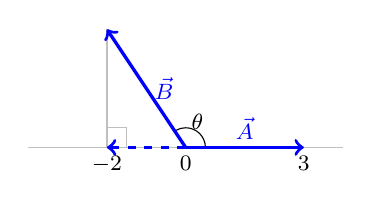
\begin{tikzpicture}[scale=0.5]\footnotesize
\draw[color=lightgray] (-4,0) -- (4,0);
\draw[color=lightgray] (-2,3) -- (-2,0);
\draw[color=lightgray] (-1.5,0) -- (-1.5,0.5) -- (-2,0.5);
\draw (0.5,0) arc (0:120:0.5);
\draw[->,very thick,color=blue] (0,0) -- (3,0);
\draw[->,very thick,color=blue] (0,0) -- (-2,3);
\draw[->,dashed,very thick,color=blue] (0,0) -- (-2,0);
\draw (0.3,0.25) node[above] {$\theta$};
\draw (1.5,0) node[above,color=blue]{$\vec{A}$};
\draw (-1,1.5) node[right,color=blue]{$\vec{B}$};
\draw (0,0) node[below] {$0$};
\draw (3,0) node[below] {$3$};
\draw (-2,0) node[below] {$-2$};
\end{tikzpicture}
\end{minipage}

\noindent On obtient bien par le calcul analytique 
le résultat obtenu par la projection géométrique.

Une autre vérification nécessaire concerne la généricité de la méthode : 
on doit pouvoir l'appliquer à d'autres exemples de produits scalaires.
C'est l'objet de la section \ref{affectation:maths:genericite} suivante.

\subsection{Généricité}\label{affectation:maths:genericite}
Pour tester la généricité de la méthode précédente, 
calculer , à l'aide du code \python{} précédent, les produits scalaires suivants :
$\vec{A}\cdot\vec{A}$, $\vec{A}\cdot\vec{C}$, $\vec{A}\cdot\vec{D}$, $\vec{A}\cdot\vec{E}$,
$\vec{C}\cdot\vec{C}$, $\vec{C}\cdot\vec{D}$, $\vec{C}\cdot\vec{E}$,
$\vec{D}\cdot\vec{D}$, $\vec{D}\cdot\vec{E}$ et $\vec{E}\cdot\vec{E}$.
Les vecteurs $\vec{A}$, $\vec{C}$, $\vec{D}$ et $\vec{E}$ sont 
définis sur la figure ci-dessous.
 $$
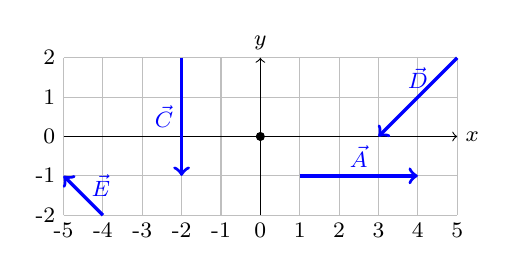
\begin{tikzpicture}[scale=0.5]\footnotesize
\draw[color=lightgray](-5,-2) grid[xstep=1,ystep=1] (5,2);
\foreach \x in {-5,-4,...,5} \draw(\x,-2) node[below]{\x};
\foreach \y in {-2,-1,...,2} \draw(-5,\y) node[left]{\y};
\filldraw(0,0) circle (0.1);
\draw[->] (-5,0) -- (5,0);
\draw (5,0) node[right]{$x$} ;
\draw[->] (0,-2) -- (0,2);
\draw (0,2) node[above]{$y$};
\draw[->,very thick,color=blue] (1,-1) -- (4,-1);
%\draw[->,very thick,color=blue] (-2,-2) -- (-4,1);
\draw[->,very thick,color=blue] (5,2) -- (3,0);
\draw[->,very thick,color=blue] (-2,2) -- (-2,-1);
\draw[->,very thick,color=blue] (-4,-2) -- (-5,-1);
\draw (2.5,-1) node[above,color=blue]{$\vec{A}$};
%\draw (-3,-0.5) node[right,color=blue]{$\vec{B}$};
\draw (-2,0.5) node[left,color=blue]{$\vec{C}$};
\draw (4,1) node[above,color=blue]{$\vec{D}$};
\draw (-4.5,-1.25) node[right,color=blue]{$\vec{E}$};
\end{tikzpicture}
$$
Vérifier en particulier qu'on obtient bien les résultats attendus pour
le produit scalaire d'un vecteur par lui-même et pour le produit scalaire 
de deux vecteurs perpendiculaires.

\subsection{Entraînement}\label{affectation:maths:entrainement} 
Dans le m\^eme esprit, utiliser l'affectation pour calculer :
\begin{enumerate}
\item le produit vectoriel $\vec{A}\times\vec{B}$ de 2 vecteurs $\vec{A}$ et $\vec{B}$
	de $\mathbb{R}^3$ de composantes respectives $(a_1,a_2,a_3)$ et $(b_1,b_2,b_3)$;
\item le produit mixte $\vec{A}\cdot(\vec{B}\times\vec{C})$ de 3 vecteurs $\vec{A}$,
	$\vec{B}$ et $\vec{C}$ de $\mathbb{R}^3$ de composantes respectives $(a_1,a_2,a_3)$, 	
	$(b_1,b_2,b_3)$ et $(c_1,c_2,c_3)$.
\end{enumerate}


%-------------------------------------------------------------------------
\section{Physique : conversion d'unités}\label{affectation:physique}
%-------------------------------------------------------------------------
\subsection{Objectif}\label{affectation:physique:objectif}
\begin{description}
\item[Principal : ] mettre en \oe uvre l'instruction d'affectation.
\item[Secondaire :] effectuer une conversion d'unités physiques.
\end{description}

\subsection{Syntaxe \python}\label{affectation:physique:python} 
\begin{description}
\item[\texttt{variable = expression}]\mbox{}
\end{description}

\subsection{Enoncé}\label{affectation:physique:enonce}
On veut convertir 3 n\oe uds marins (miles nautiques par heure) en kilomètres par heure (km/h).\\
Proposer une instruction de type « affectation » qui permettra de réaliser cette conversion.

\subsection{Méthode}\label{affectation:physique:methode}
Pour expliciter la méthode qui nous permettra de résoudre un ensemble de problèmes 
équivalents et en particulier le problème posé dans l'énoncé, on commence par s'abstraire 
des données spécifiques, en particulier numériques, pour ne considérer que les variables associées. 
Ainsi, on ne s'intéressera pas au nombre de n\oe uds (3) à convertir, ni d'ailleurs aux n\oe uds
eux-mêmes ou encore aux kilomètres par heure mais plutôt à ce qu'ils qualifient : deux unités 
physiques compatibles et une certaine quantité de l'une d'entre elles.

On cherche donc ici à convertir $n_1\cdot u_1$ en $n_2\cdot u_2$ 
où $u_1$ et $u_2$ sont des unités physiques compatibles 
qui dérivent de la même unité de base $u_b$ du \href{http://www.bipm.org/fr/si/}{Système international d'unités}.
$$\left|\begin{array}{l@{\ =\ }r}
u_1 & a_1\cdot u_b \\
u_2 & a_2\cdot u_b
\end{array}\right.
\ \Rightarrow\ \ 
\left|\begin{array}{l@{\ =\ }r@{\ =\ }r}
n_1\cdot u_1 & n_1\cdot (a_1\cdot u_b) & (n_1\cdot a_1)\cdot u_b\\
n_2\cdot u_2 & n_2\cdot (a_2\cdot u_b) & (n_2\cdot a_2)\cdot u_b
\end{array}\right.
\ \Rightarrow\ \ \frac{n_1\cdot u_1}{n_2\cdot u_2} = \frac{n_1\cdot a_1}{n_2\cdot a_2}$$
Comme on cherche $n_2$ tel que $n_1\cdot u_1 = n_2\cdot u_2$, on a donc :
$$\frac{n_1\cdot u_1}{n_2\cdot u_2} = \frac{n_1\cdot a_1}{n_2\cdot a_2} = 1
\ \Rightarrow\ \ n_2 = n_1 \cdot \frac{a_1}{a_2}$$
où les coefficients $a_i$ sont documentés dans le Système international d'unités par le
\href{http://www.bipm.org/}{Bureau international des poids et mesures}.

Une fois connus les coefficients $a_i$, on détermine la quantité $n_2$ de l'unité $u_2$
par une affectation simple : \texttt{n2 = n1*a1/a2} .

\subsection{Résultat} On applique la méthode précédente à la conversion
proposée dans l'énoncé où $u_1$ représente les n\oe uds (miles nautiques par heure), 
$u_2$ les kilomètres par heure (km/h) et $u_b$ les mètres par seconde (m/s).
Le Système international d'unités fournit par ailleurs les facteurs 
de conversion $a_1$ (nd $\rightarrow$ m/s) et $a_2$ (km/h $\rightarrow$ m/s) :
$a_1 = 1852/3600$ et $a_2 = 1000/3600$.


\noindent\begin{minipage}{7cm}
Compte-tenu de ces valeurs, le code ci-contre
permet de calculer le nombre $n_2$ de kilomètres par heure
en fonction du nombre $n_1$ de n\oe uds.
\end{minipage}
\hfill
\begin{minipage}{8cm}
\begin{lstlisting}[caption=\textbf{conversion d'unités}]
a1 = 1852/3600
a2 = 1000/3600
n2 = n1*a1/a2
\end{lstlisting}
\end{minipage}

Remarque : on n'a pas cherché à effectuer « à la main » les calculs numériques :
\python{} les fera mieux que nous; et surtout, on n'a pas cherché non plus à 
particulariser la $3^{\grave eme}$ ligne du code en \texttt{n2 = n1*1852/1000} :
la forme plus abstraite \texttt{n2 = n1*a1/a2} restera identique pour convertir 
des parsecs en années-lumière (longueurs), des gallons en barils (volumes) ou 
encore des électron-volts en frigories (énergies), seules les valeurs des coefficients $a_i$ changeront (lignes \texttt{1} 
et \texttt{2} du code).

\subsection{Vérification}\label{affectation:physique:verification}
Pour vérifier le résultat précédent, on peut comparer les valeurs obtenues par le calcul 
avec celles de quelques valeurs caractéristiques facilement évaluables « à la main »
(exemples : $n_1 = 1\ \rm{nd} \Rightarrow{} n_2 = 1.852\ \rm{km/h}$ ou
$n_1 = 1/1852\ \rm{nd} \Rightarrow{} n_2 = 1/1000\ \rm{km/h}$).

\begin{minipage}[t]{7.5cm}\footnotesize
\begin{Verbatim}
>>> n1 = 1
>>> a1, a2 = 1852/3600, 1000/3600
>>> n2 = n1*a1/a2
>>> n2
1.852
\end{Verbatim}
\end{minipage}
\hfill
\begin{minipage}[t]{7.5cm}\footnotesize
\begin{Verbatim}
>>> n1 = 1/1852
>>> a1, a2 = 1852/3600, 1000/3600
>>> n2 = n1*a1/a2
>>> n2
0.0010000000000000002
\end{Verbatim}
\end{minipage}
\vspace*{2mm}

\noindent On obtient bien par le calcul les résultats escomptés.

Une autre vérification nécessaire concerne la généricité de la méthode : 
on doit pouvoir l'appliquer à d'autres exemples de conversion d'unités.
C'est l'objet de la section \ref{affectation:physique:genericite} suivante.

\subsection{Généricité}\label{affectation:physique:genericite}
Pour tester la généricité de la méthode précédente, 
effectuer, à l'aide du code \python{} précédent, les conversions suivantes 
en s'appuyant sur le \href{http://www.bipm.org/fr/si/}{Système international d'unités} :
\begin{enumerate}
\item des parsecs en années-lumière,
\item des gallons en barils,
\item des électron-volts en frigories.
\end{enumerate}

\subsection{Entraînement}\label{affectation:physique:entrainement}
Dans le même esprit, et en s'appuyant à nouveau sur le 
\href{http://www.bipm.org/fr/si/}{Système international d'unités}, 
utiliser l'affectation pour convertir :
\begin{enumerate}
\item une température \bsc{Fahrenheit} ($^\circ$F) en une température \bsc{Celsius} ($^\circ$C).
\item une température \bsc{Rankine} ($^\circ$Ra) en une température \bsc{Celsius} 	($^\circ$C).
\end{enumerate}

%-------------------------------------------------------------------------
\section{Informatique : préfixes binaires}\label{affectation:informatique}
%-------------------------------------------------------------------------

\subsection{Objectif}\label{affectation:informatique:objectif}
\begin{description}
\item[Principal : ] mettre en \oe uvre l'instruction d'affectation.
\item[Secondaire :] manipuler les puissances décimales et binaires de l'unité d'information.
\end{description}

\subsection{Syntaxe \python}\label{affectation:informatique:python}
\begin{description}
\item[\texttt{variable = expression}]\mbox{}
\item[\texttt{x**n}] calcule $x^n$.
\end{description}

\subsection{Enoncé}\label{affectation:informatique:enonce}
Un bit est un chiffre binaire (\emph{binary digit} : 0 ou 1). 
C'est l'unité élémentaire d'information. 
Un octet (\emph{byte}) est une unité d'information composé de 8 bits.\\
Proposer une instruction de type « affectation » qui permettra de déterminer 
le nombre d'octets dans 1 Go (1~giga-octet).

\subsection{Méthode}\label{affectation:informatique:methode}
En informatique, on parle souvent de kilo-octets (ko), méga-octets (Mo), 
giga-octets (Go), téra-octets (To) et autres péta-octets (Po). 
L'idée est donc ici est de savoir comment calculer ces différentes unités
en fonction de l'octet.

Les préfixes kilo, méga, giga, téra, péta\ldots\  sont définis par le 
\href{http://www.bipm.org/fr/si/}{Système international d'unités}
comme des puissances de $10^3$. 
En 1998, la
\href{http://www.electropedia.org/iev/iev.nsf/display?openform&ievref=112-01-27}{Commission Electrotechnique Internationale} institua les préfixes binaires plus adaptés à l'Informatique.
Ce sont en fait des puissances de $2^{10}$ appelées kibi-octet, mébi-octet, 
gibi-octet, tébi-octet, pébi-octet\ldots\ (Table \ref{fig:informatique:prefixes}).

\begin{table}[ht]
$$\begin{tabular}{|lr|c|c|c|c|c|c|c|c|}
\cline{3-10}
\multicolumn{2}{l|}{} & \multicolumn{8}{c|}{\textbf{préfixes multiplicateurs}}\\
\cline{3-10}
\multicolumn{2}{r|}{\tiny préfixes décimaux} & kilo		& méga		& giga		& téra 		& péta 		& exa		& zetta		& yotta \\
\multicolumn{2}{r|}{\tiny symboles} & \tiny ko & \tiny Mo & \tiny Go & \tiny To & \tiny Po & \tiny Eo & \tiny Zo & \tiny Yo \\
\multicolumn{2}{r|}{\tiny$n$} & \tiny 1 & \tiny 2 & \tiny 3 & \tiny 4 & \tiny 5 & \tiny 6 & \tiny 7 & \tiny 8 \\
\hline
 & & & & & & & & & \\[-3mm]
décimal	& $(10^{3})^n$  	& $10^{3}$  & $10^{6}$	& $10^{9}$	& $10^{12}$	& $10^{15}$ & $10^{18}$	& $10^{21}$	& $10^{24}$\\
 & & & & & & & & & \\[-3mm]
binaire & $(2^{10})^n$  	& $2^{10}$  & $2^{20}$	& $2^{30}$	& $2^{40}$	& $2^{50}$ 	& $2^{60}$	& $2^{70}$	& $2^{80}$\\
\hline
\multicolumn{2}{r|}{\tiny$n$} & \tiny 1 & \tiny 2 & \tiny 3 & \tiny 4 & \tiny 5 & \tiny 6 & \tiny 7 & \tiny 8 \\
\multicolumn{2}{r|}{\tiny symboles} & \tiny Kio & \tiny Mio & \tiny Gio & \tiny Tio & \tiny Pio & \tiny Eio & \tiny Zio & \tiny Yio \\
\multicolumn{2}{r|}{\tiny préfixes binaires} & kibi		& mébi		& gibi		& tébi 		& pébi 		& exbi		& zebi		& yobi \\
\cline{3-10}
\end{tabular}$$
\caption{Préfixes multiplicateurs en décimal et en binaire}
\label{fig:informatique:prefixes}
\end{table}

Ainsi, le préfixe $p$ prendra la forme $p = f^n$ où $f$ est le facteur multiplicatif qui vaut $10^3$
dans le système décimal et $2^{10}$ dans le système binaire, et $n$ la puissance recherchée
($n=1$ pour kilo ou kibi, $n=2$ pour méga ou mébi\ldots) : \texttt{prefixe = facteur**n}.

\subsection{Résultat}\label{affectation:informatique:resultat}
On applique la méthode précédente aux giga-octets (qu'on devrait appeler des gibi-octets) :
$n = 3$ et $f = 2^{10}$.

\noindent\begin{minipage}{7cm}
Compte-tenu de ces valeurs, le code \python{} ci-contre
permet de calculer le nombre d'octets dans un giga-octet.
\end{minipage}
\hfill
\begin{minipage}{8cm}
\begin{lstlisting}[caption=\textbf{giga-octets ou gibi-octets}]
n = 3
facteur = 2**10
prefixe = facteur**n
\end{lstlisting}
\end{minipage}

Remarque : on n'a pas cherché à effectuer « à la main » les calculs numériques :
\python{} les fera mieux que nous; et surtout, on n'a pas cherché non plus à 
particulariser la $3^{\grave eme}$ ligne du code en \texttt{prefixe = (2**10)**3} :
la forme plus abstraite \texttt{prefixe = facteur**n} restera identique pour calculer
aussi bien en décimal qu'en binaire des yotta-octets ou des yobi-octets, 
seules les valeurs de \texttt{facteur} et de \texttt{n} changeront (lignes \texttt{1} 
et \texttt{2} du code).

\subsection{Vérification}\label{affectation:informatique:verification}
Pour vérifier le résultat précédent, on pourra se référer au site officiel de la
\href{http://www.electropedia.org/iev/iev.nsf/display?openform&ievref=112-01-27}{Commission Electrotechnique Internationale}.
On y vérifie bien que 1 Gio = 1 073 741 824 octets alors que 1~Go~=~1 000 000 000 octets.
Dans la pratique, on parle toujours de kilo-, méga- ou giga-octets 
tout en faisant référence aux kibi-, mébi ou gibi-octets.

\begin{minipage}[t]{7.5cm}\footnotesize
\begin{Verbatim}
>>> n = 3
>>> facteur = 2**10
>>> prefixe = facteur**n
>>> prefixe
1073741824
\end{Verbatim}
\end{minipage}
\hfill
\begin{minipage}[t]{7.5cm}\footnotesize
\begin{Verbatim}
>>> n = 3
>>> facteur = 10**3
>>> prefixe = facteur**n
>>> prefixe
1000000000
\end{Verbatim}
\end{minipage}
\vspace*{2mm}

Une autre vérification nécessaire concerne la généricité de la méthode : 
on doit pouvoir l'appliquer à d'autres exemples de préfixes binaires.
C'est l'objet de la section \ref{affectation:informatique:genericite} suivante.

\subsection{Généricité}\label{affectation:informatique:genericite}
Pour tester la généricité de la méthode précédente, calculer, à l'aide du code \python{} précédent,
les valeurs en octets des préfixes suivants :

\begin{minipage}[t]{7.5cm}
\begin{enumerate}
\item kibi
\item mébi
\end{enumerate}
\end{minipage}
\hfill
\begin{minipage}[t]{7.5cm}
\begin{enumerate}\setcounter{enumi}{2}
\item tébi
\item pébi
\end{enumerate}
\end{minipage}

\subsection{Entraînement}\label{affectation:informatique:entrainement}
Dans le même esprit, proposer une instruction de type « affectation » qui permettra 
de déterminer les différences entre les préfixes décimaux et binaires correspondants.

\begin{minipage}[t]{7.5cm}
\begin{enumerate}
\item kilo-kibi
\item méga-mébi
\item giga-gibi
\end{enumerate}
\end{minipage}
\hfill
\begin{minipage}[t]{7.5cm}
\begin{enumerate}\setcounter{enumi}{3}
\item téra-tébi
\item péta-pébi
\item yotta-yobi
\end{enumerate}
\end{minipage}

%-------------------------------------------------------------------------
\section{Retours d'expériences}\label{affectation:retours}
%-------------------------------------------------------------------------

%-------------------------------------------------------------------------
\subsection{Algorithmes}\label{affectation:retours:algorithmes}


%-------------------------------------------------------------------------
\subsection{\mrv : méthode}\label{affectation:retours:methode}

Etant donné un énoncé qui propose de résoudre un exercice
portant sur un cas particulier donné, la première étape de la démarche \textsc{Mrv} consiste à
décrire une méthode générique qui, lorsqu'on l'appliquera, permettra de résoudre 
le cas particulier considéré ainsi que tout problème équivalent à celui 
qui est posé.

Pour expliciter une telle méthode générique, on a commencé par s'abstraire 
des données spécifiques, en particulier numériques et alphanumériques, 
pour ne considérer que les variables associées. 
Puis, on a exprimé
la solution \texttt{s} recherchée sous la forme d'une fonction \texttt{f} 
des données \texttt{x1}, \texttt{x2}\ldots{} abstraites du problème :
\texttt{s = f(x1,x2,...,xn)}.

L'association systématique de noms à des valeurs constitue ainsi un premier
moyen d'abstrac\-tion qui permet de ne pas faire appel aux
données spécifiques à un problème particulier
dans l'élabora\-tion de la méthode générique.

%-------------------------------------------------------------------------
\subsection{\mrv : résultat}\label{affectation:retours:resultat}

Etant donné une méthode générique pour résoudre un ensemble de problèmes 
équivalents, le deuxième étape de la démarche \textsc{Mrv} consiste à
appliquer cette méthode à un problème particulier.

Ayant fait abstraction des valeurs particulières dans l'explicitation 
de la méthode générique, appliquer la méthode a consisté ici à attribuer
ces valeurs particulières aux différentes variables qui interviennent 
dans la détermination de la solution recherchée. 
En effet, dans les exercices précédents sur l'affectation,
la solution \texttt{s} recherchée a toujours pris la forme
\texttt{s = f(x1,x2,...,xn)}. La fonction \texttt{f}
ayant été déterminée par la première étape de la démarche \textsc{Mrv},
il ne reste plus qu'à donner des valeurs aux variables \texttt{x1}, \texttt{x2}\ldots{} 
pour être capable d'évaluer le membre de droite \texttt{f(x1,x2,...,xn)} de l'affectation
et donc la solution \texttt{s}, membre de gauche de cette affectation.

On passe ainsi d'un cas particulier à un autre en changeant simplement les valeurs
des données spécifiques aux problèmes particuliers.

%-------------------------------------------------------------------------
\subsection{\mrv : vérification}\label{affectation:retours:verification}

\paragraph{Vérification du résultat :}
Etant donné un résultat obtenu par application d'une méthode générique pour résoudre un problème particulier, la troisième étape de la démarche \textsc{Mrv} consiste à vérifier ce résultat
par des méthodes alternatives ou complémentaires de celle déjà utilisée.

Les exemples précédents ont mis en \oe uvre tout un éventail de méthodes pour vérifier
les résultats obtenus :
\begin{itemize}
\item des méthodes alternatives qui calculent la solution
	par une autre voie comme 
	le calcul du produit scalaire par une méthode géométrique 
	(\ref{affectation:maths:verification}) ou
	le calcul de distance par un logiciel éprouvé :
	le module \texttt{turtle} de \python{} (\ref{affectation:figures:verification});
\item la reconstruction des données à partir des résultats obtenus
	comme pour le calcul du quotient et du reste de la division entière
	(\ref{affectation:nombres:verification});
\item des jeux de tests comme pour 
	le lancer de dés (\ref{affectation:jeux:verification}) ou 
	la conversion d'unités (\ref{affectation:physique:verification});
\item l'estimation d'un ordre de grandeur comme dans 
	le prix d'un livre (\ref{affectation:vie-courante:verification})
	ou de simples calculs « à la main » lorsque c'est possible
	comme pour les chaînes de caractères (\ref{affectation:textes:verification});
\item la consultation d'un ouvrage de référence reconnu comme dans le cas 
	des préfixes binaires (\ref{affectation:informatique:verification}).
\end{itemize}


L'application de ces différentes méthodes de vérification ne prouve pas formellement 
que les résultats obtenus sont corrects, mais renforce ou non la confiance que l'on 
peut en avoir. 
L'une ou l'autre de ces méthodes pourra être reprise, avec d'autres qui apparaîtrons au fur 
et à mesure des chapitres suivants, pour vérifier systématiquement les résultats des exercices.
Le cas particulier de la méthode par jeux de tests sera même systématiquement intégré
dans la spécification des fonctions (partie \ref{fonctions}, chapitre \ref{fonctions:specification}).

\paragraph{Vérification de la méthode :}
Il reste à tester la généricité de la méthode en l'appliquant
à des exemples différents relevant du même type de problème.
C'est ce qui a été systématiquement réalisé pour chacun des exemples traités
(\ref{affectation:vie-courante:genericite}, \ref{affectation:jeux:genericite}, 
\ref{affectation:textes:genericite}, \ref{affectation:nombres:genericite}, 
\ref{affectation:figures:genericite}, \ref{affectation:maths:genericite}, 
\ref{affectation:physique:genericite}, \ref{affectation:informatique:genericite}).
